\section{Panoramamottagare}
\index{panoramamottagare}
\index{mottagare!panorama}
\index{spektrumanalysator}

\begin{figure}
  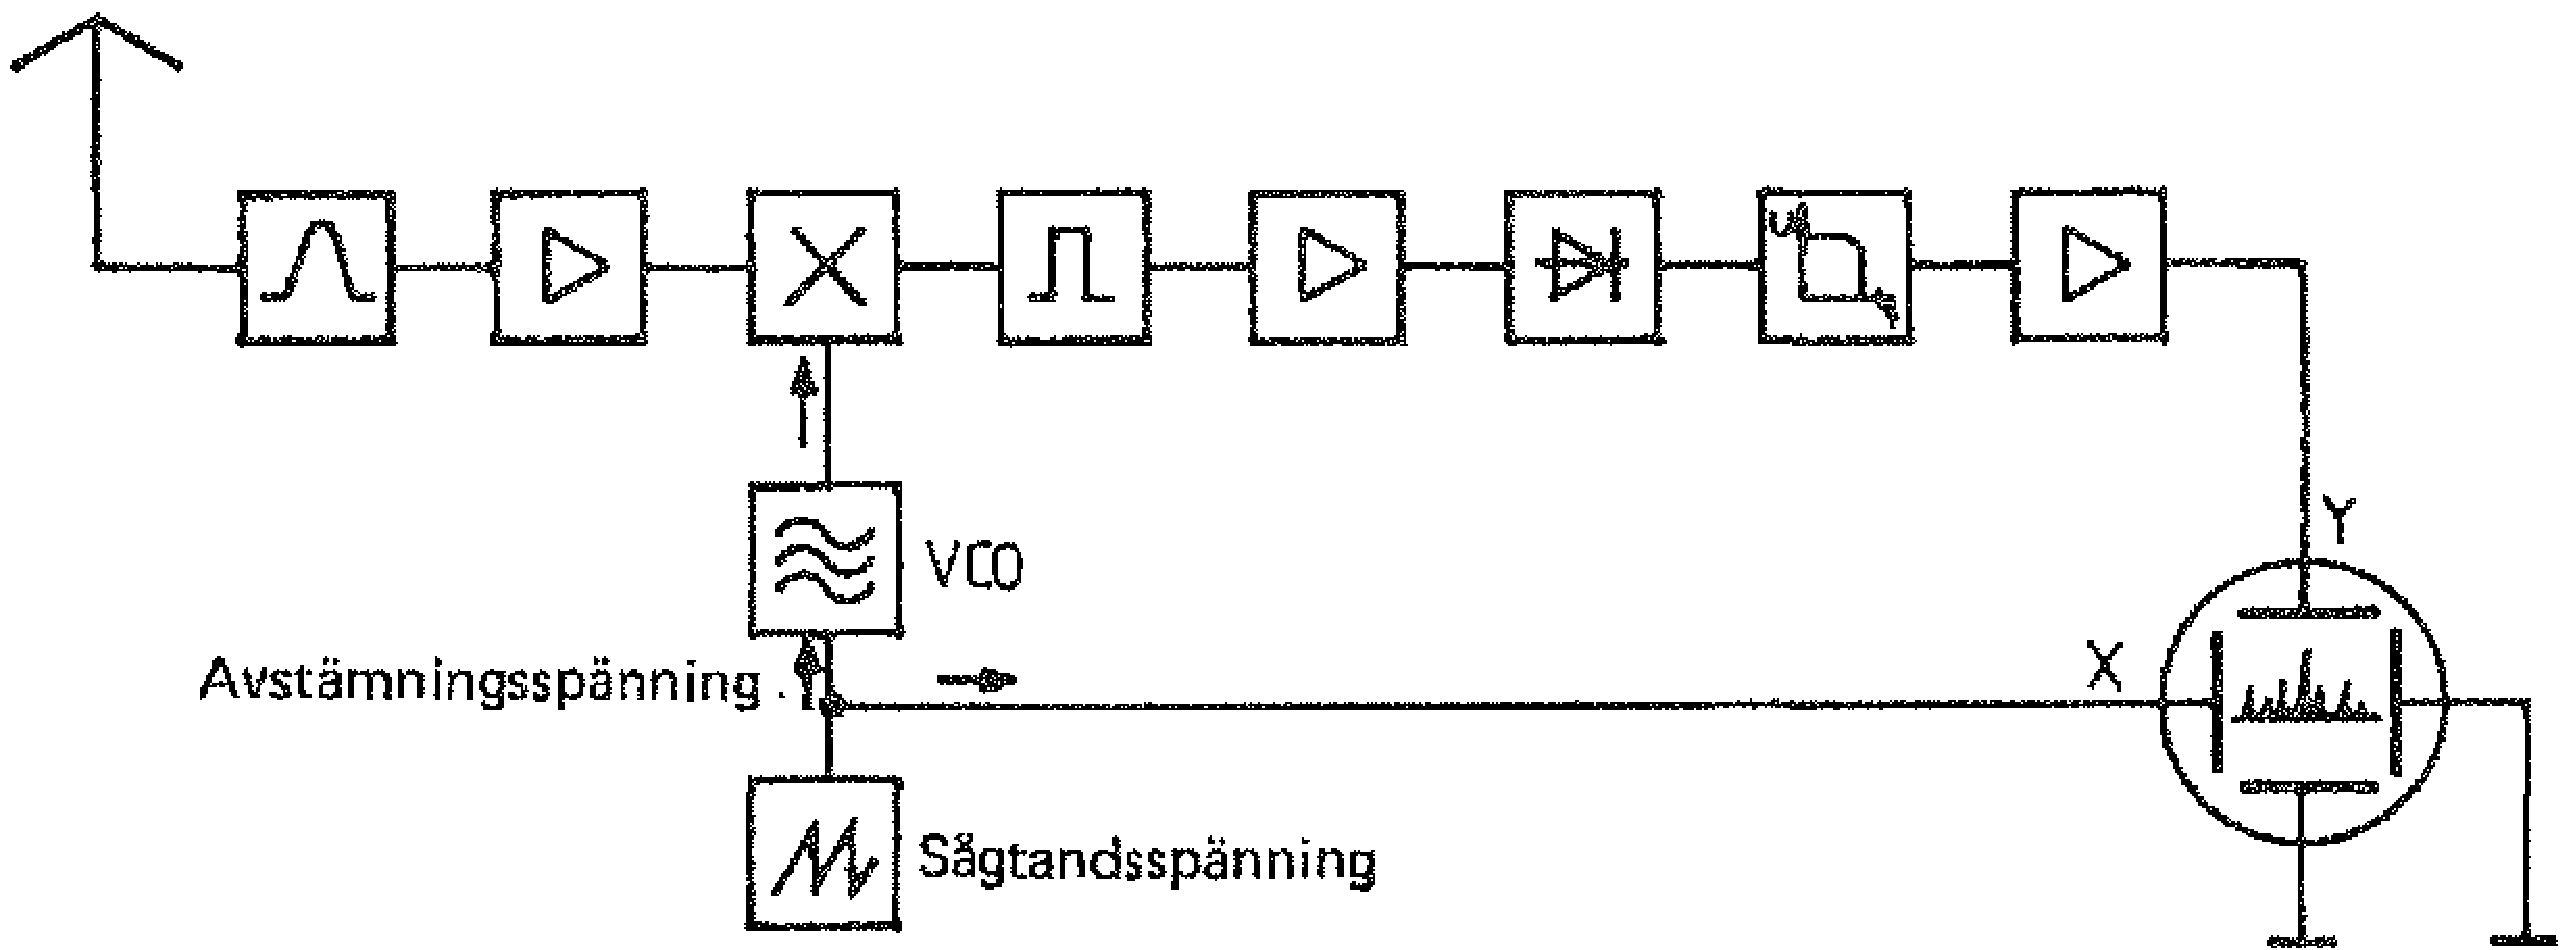
\includegraphics[width=\textwidth]{images/cropped_pdfs/bild_2_4-15.pdf}
  \caption{Panoramamottagare}
  \label{fig:bildII4-15}
\end{figure}

I en \emph{panoramamottagare} (eng. \emph{panorama receiver}) eller
\emph{spektrumanalysator} (eng. \emph{spectrum analyzer}) visas på en
oscilloskopskärm var det finns signaler inom ett frekvensband, som illustreras
i bild \ref{fig:bildII4-15}.
En panoramamottagare är en superheterodyn.
Ofta implementeras de så att de sveper över mellanfrekvensen på en mottagare,
och hjälper därmed till att se vad som finns i angränsande del av bandet innan
det filtrerats för smalt.
Detta hjälper till att identifiera närliggande störkällor så väl som andra
potentiella stationer att köra QSO med.

\begin{wrapfigure}{R}{0.5\textwidth}
  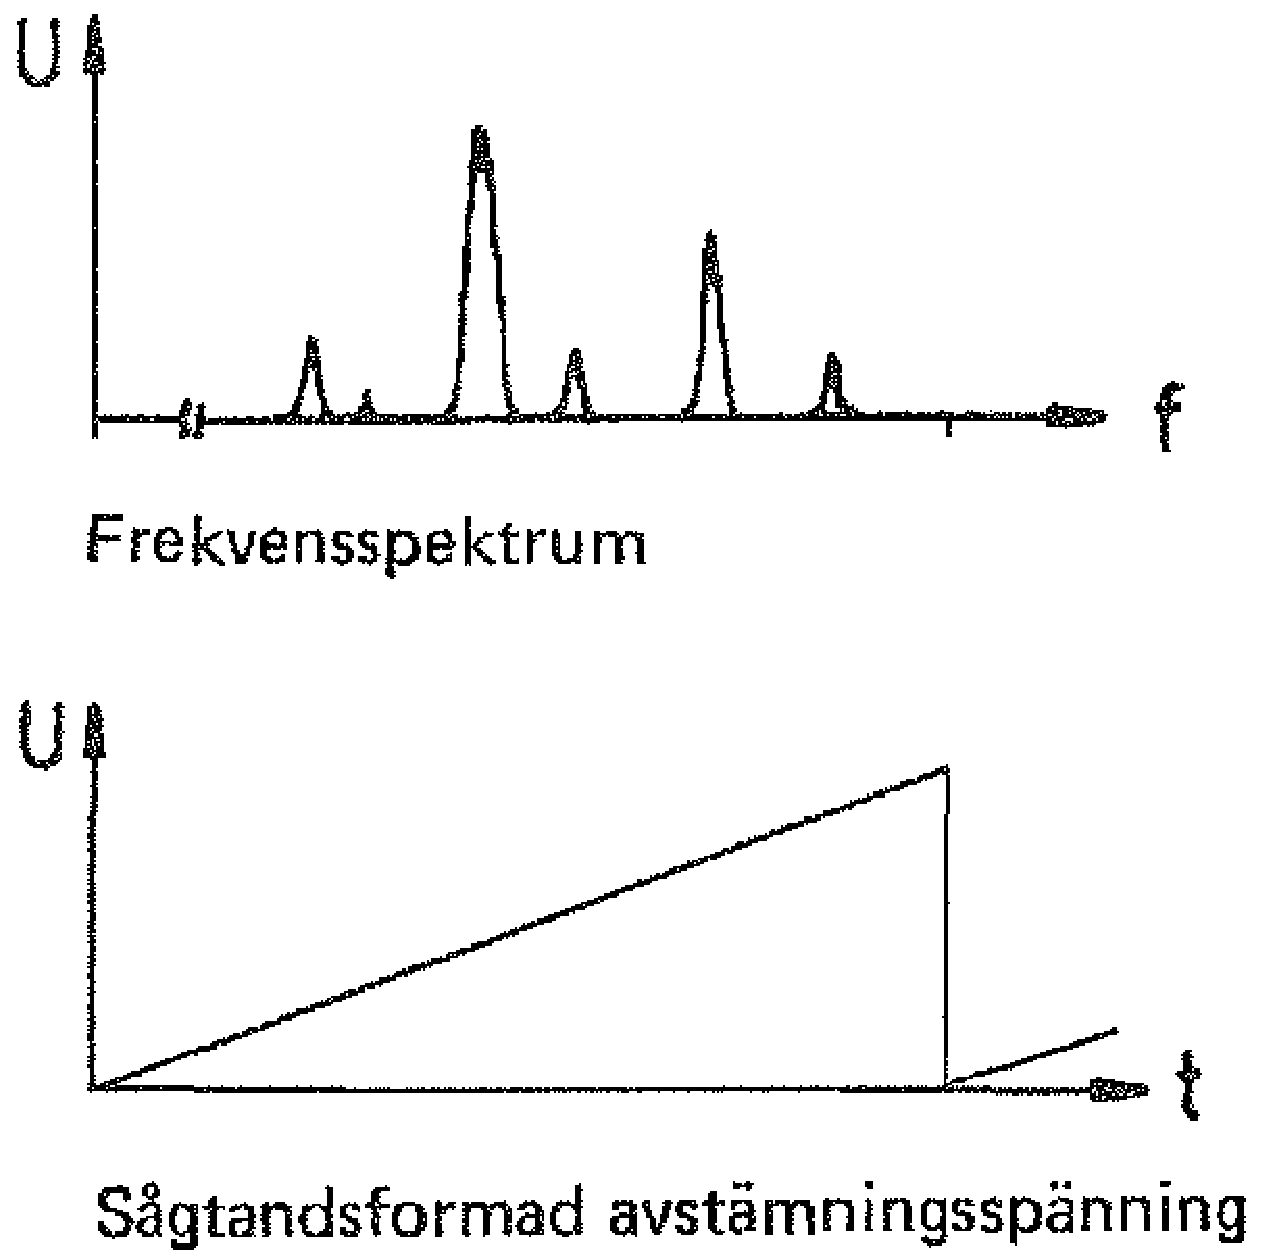
\includegraphics[width=0.5\textwidth]{images/cropped_pdfs/bild_2_4-17.pdf}
  \caption{Signal- och svepspänningar}
  \label{fig:bildII4-17}
\end{wrapfigure}

Bild \ref{fig:bildII4-17} illustrerar frekvenssvepet över spektrat.
Mottagaroscillatorn är en VCO (spänningsstyrd oscillator).
Dennas frekvens styrs av en sågtandformad likspänning, som stiger linjärt för
att snabbt falla tillbaka och återupprepas.
VCO sveper då över det önskade frekvensbandet med ett antal gånger per sekund.
Med samma sågtandspänning avlänkas strålen på skärmen utmed x-axeln.

Den mottagna signalen demoduleras och översätts till en likspänning
som skildrar de mottagna signalernas styrka.
Med denna likspänning avlänkas strålen på bildskärmen utmed y-axeln.
Strålens avstånd från x-axeln anger alltså den mottagna stationens styrka
och strålens läge utmed x-axeln anger var stationen ligger i det
frekvensområde som avsöks.
Beroende på hur stort frekvenssving som ges VCO, så kommer ett större eller
mindre frekvensområde att avsökas och visas på skärmen.
Området kan vara så brett som ett amatörband eller mer och ner till några
få kHz.

Utöver övervakning av ett frekvensband kan en panoramamottagare användas för
studium till exempel av signaler och sidofrekvenser som alstras i den egna stationen.
För noggranna mätningar behövs emellertid ett hjälpmedel av högre kvalitet,
kallat \emph{spektrumanalysator}.
En sådan arbetar i grunden på samma sätt som en panoramamottagare.

En panoramamottagare kan anslutas till en mottagare för att studera
signalerna inom MF-passbandet, så som visas i bild \ref{fig:bildII4-16}.
Då är mottagningsfrekvensen i bildskärmens mitt.
Stationerna under och över i frekvens visas till vänster respektive höger
om den egna frekvensen.

Vid ändrad mottagningsfrekvens blir denna fortfarande kvar mitt på skärmen.

\begin{figure}
  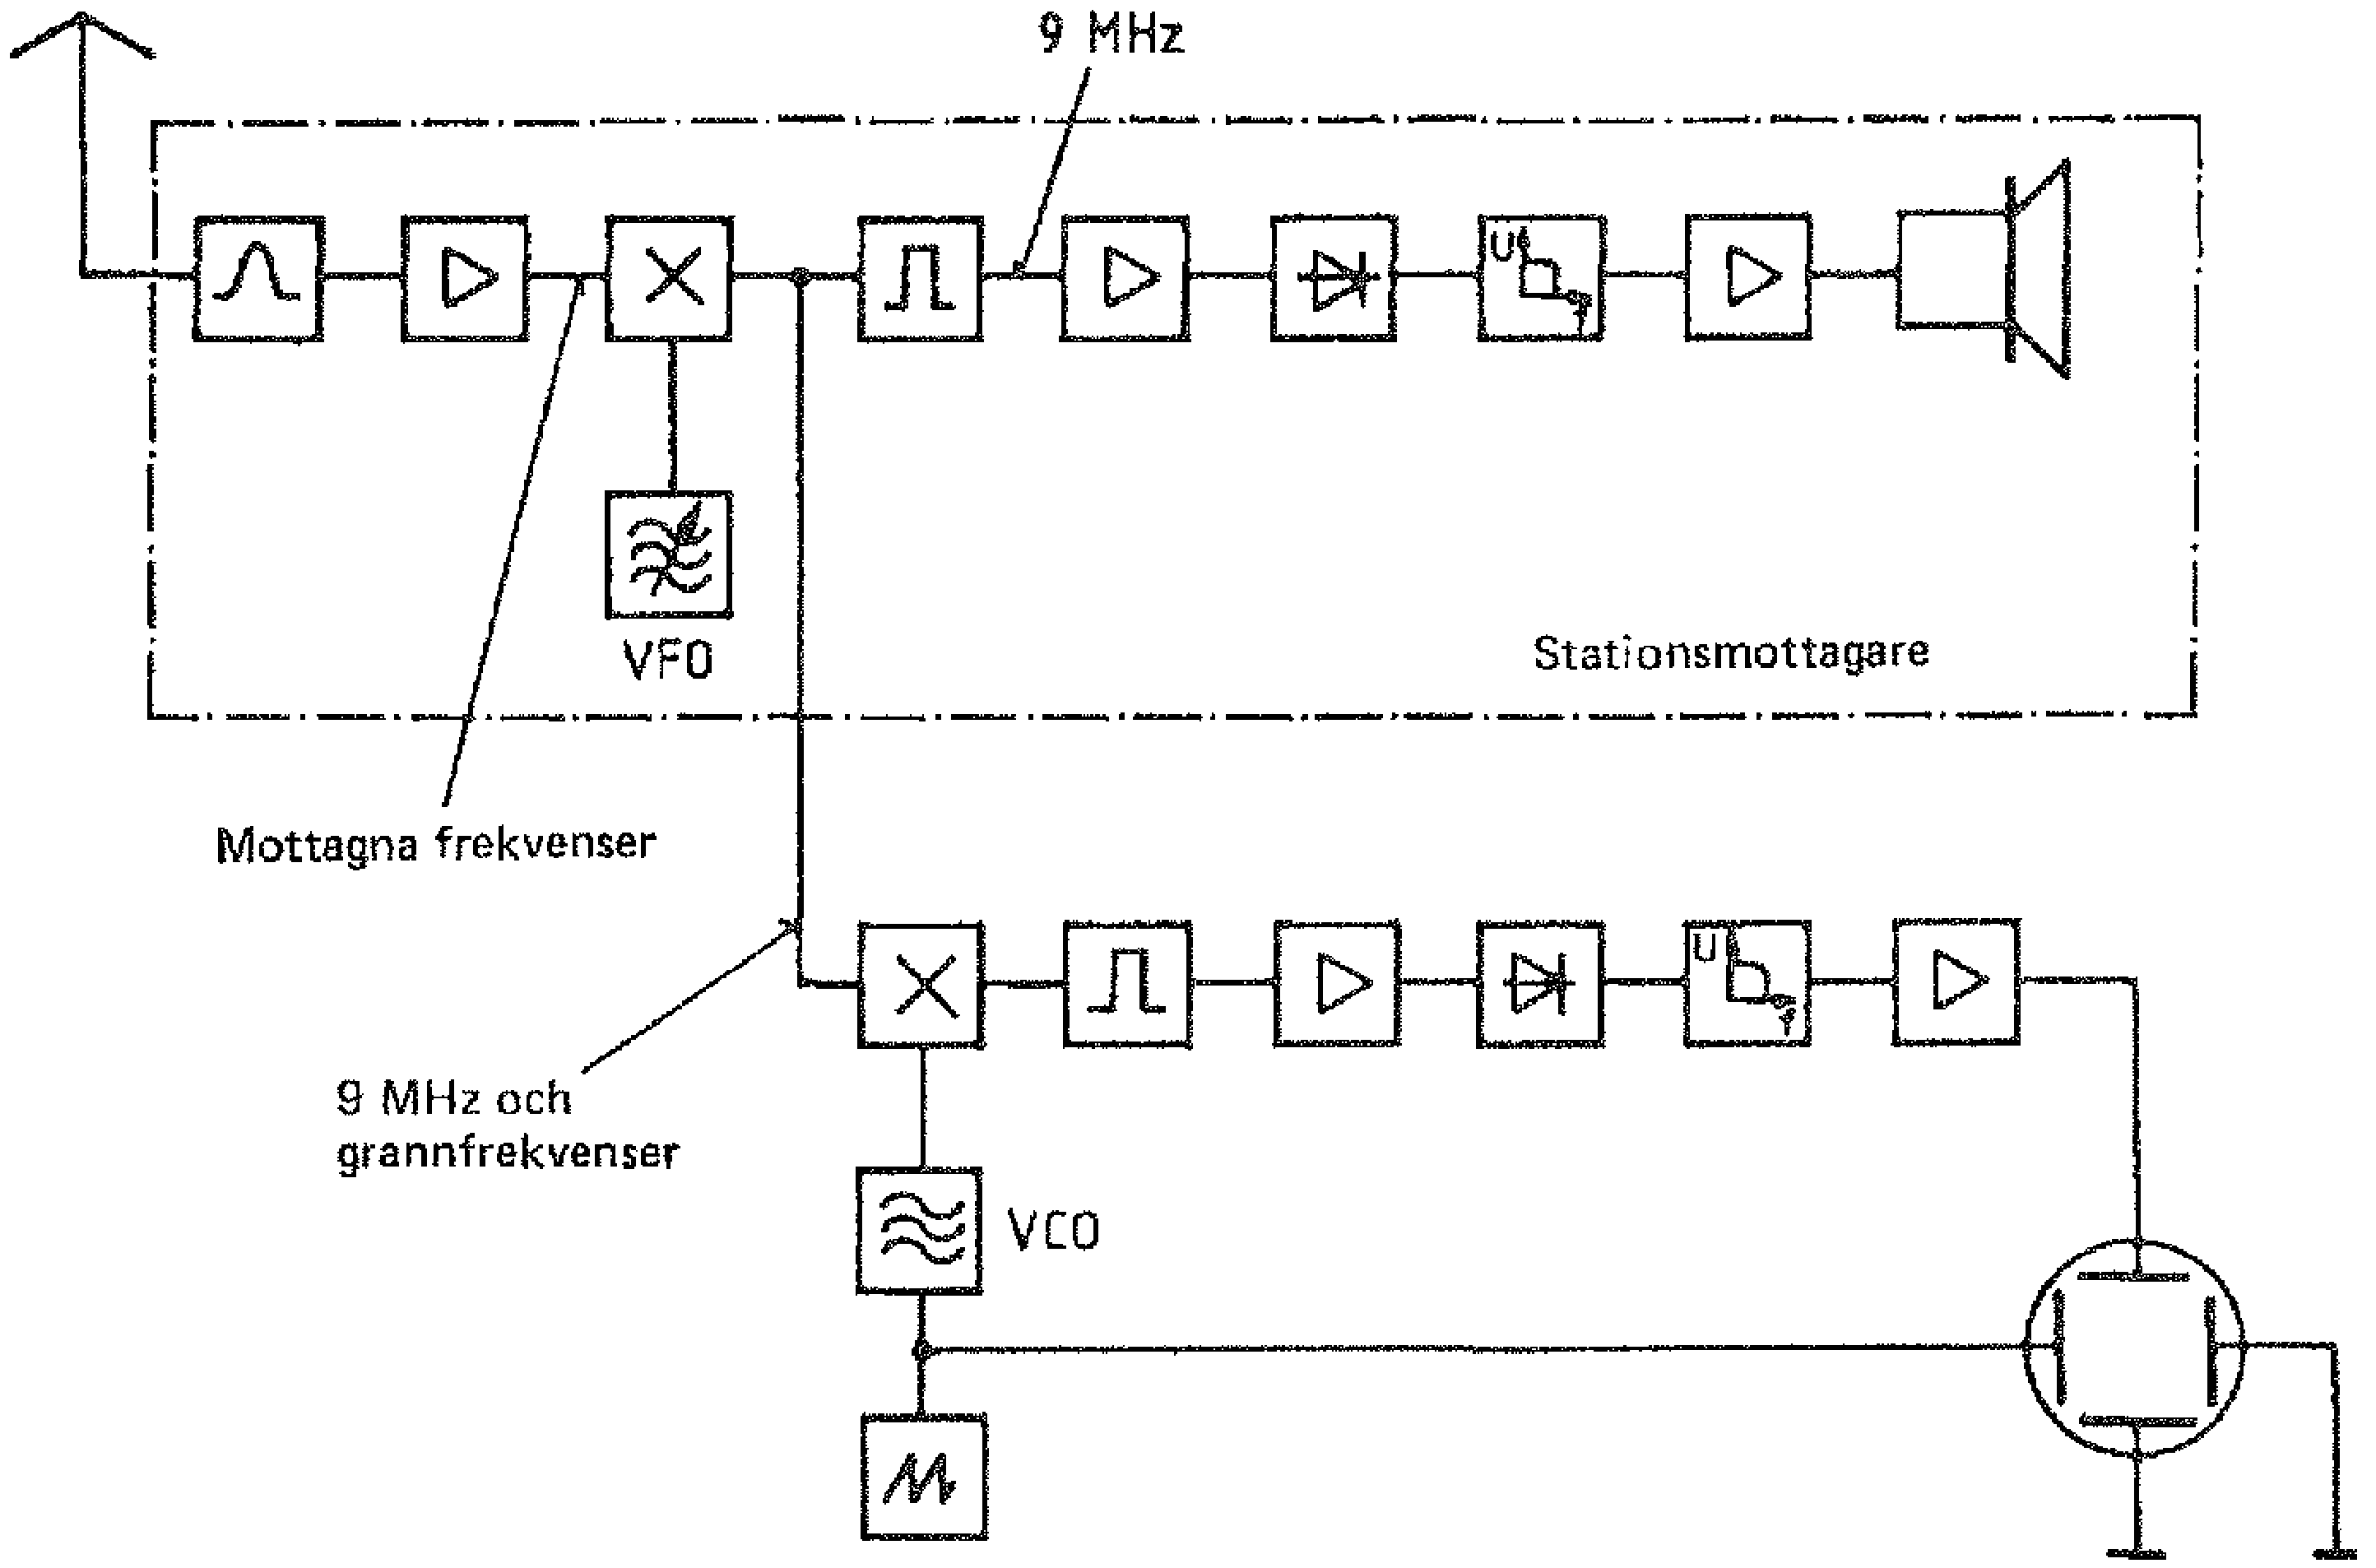
\includegraphics[width=\textwidth]{images/cropped_pdfs/bild_2_4-16.pdf}
  \caption{Anslutning av panoramamottagare till stationsmottagare}
  \label{fig:bildII4-16}
\end{figure}
